% Author: Izaak Neutelings (October 2021)
% Inspiration
%   "Very special relativity - An illustrated guide", Sander Bais (2007)
\documentclass[border=3pt,tikz]{standalone}
\usepackage{tikz}
\usepackage{amsmath} % for \text
\usepackage{etoolbox} % ifthen
\usepackage[outline]{contour} % glow around text
\usetikzlibrary{decorations.markings,decorations.pathmorphing}
\usetikzlibrary{angles,quotes} % for pic (angle labels)
\usetikzlibrary{arrows.meta} % for arrow size
\usepackage{xfp} % higher precision (16 digits?)
\contourlength{1.1pt}

\newcommand{\calI}{\mathscr{I}} %\mathcal
\tikzset{>=latex} % for LaTeX arrow head
\colorlet{myred}{red!80!black}
\colorlet{myblue}{blue!80!black}
\colorlet{mygreen}{green!80!black}
\colorlet{mydarkred}{red!55!black}
\colorlet{mydarkblue}{blue!50!black}
%\colorlet{mylightblue}{blue!60!black!30}
\colorlet{mypurple}{blue!40!red!80!black}
\colorlet{mydarkgreen}{green!50!black}
\colorlet{mydarkpurple}{blue!40!red!50!black}
%\colorlet{mylightpurple}{mydarkpurple!80!red!6}
\colorlet{myorange}{orange!40!yellow!95!black}
\colorlet{mydarkorange}{orange!40!yellow!85!black}
\tikzstyle{world line}=[myblue!60,line width=0.4]
\tikzstyle{world line t}=[mypurple!60,line width=0.4]
\tikzstyle{world line'}=[mydarkred!60,line width=0.4]
\tikzstyle{mysmallarr}=[-{Latex[length=3,width=2]},thin]
\tikzstyle{mydashed}=[dash pattern=on 3 off 3]
\tikzstyle{vector}=[->,line width=1,line cap=round]
\tikzstyle{vector'}=[vector,shorten >=1.2]
%\tikzstyle{measure}=[{Latex[length=3,width=2]}-{Latex[length=3,width=2]},thin]
\tikzstyle{particle}=[mygreen,line width=0.9]
\tikzstyle{photon}=[-{Latex[length=5,width=4]},myorange,line width=0.8,decorate,
                    decoration={snake,amplitude=1.0,segment length=5,post length=5}]

\def\tick#1#2{\draw[thick] (#1) ++ (#2:0.06) --++ (#2-180:0.12)}
\def\tickp#1#2{\draw[thick,mydarkred] (#1) ++ (#2:0.06) --++ (#2-180:0.12)}
\def\Nsamples{40} % number samples in plot

\begin{document}


% SPACETIME DIAGRAM
\begin{tikzpicture}[scale=1.8]
  \message{Basic spacetime diagram^^J}
  
  \def\xmax{2}
  \def\Nlines{4} % number of world lines (at constant x/t)
  
  % AXES
  \draw[->,thick] (0,-0.5) -- (0,\xmax+0.2) node[left=-1] {$ct  \, \, [ \si{m} ]$};
  \draw[->,thick] (-0.5,0) -- (\xmax+0.2,0) node[below=0] {$x  \, \, [ \si{m} ]$};
  
\end{tikzpicture}


% SPACETIME DIAGRAM with WORLD LINES
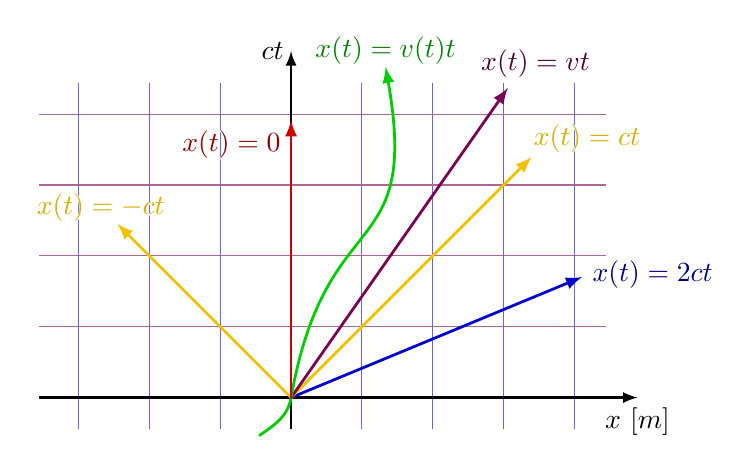
\begin{tikzpicture}[scale=2.0]
  \message{Worldlines^^J}
  
  \def\ymin{0.2}
  \def\xmin{1.6}
  \def\xmax{2}
  \def\Nlines{4} % number of world lines (at constant x/t)
  \pgfmathsetmacro\d{0.9*\xmax/\Nlines} % grid size
  \coordinate (O) at (0,0);
  \coordinate (T) at (0,\xmax+0.2);
  
  % WORLD LINES GRID
  \message{Making world lines...^^J}
  \foreach \i [evaluate={\x=\i*\d;}] in {1,...,\Nlines}{
    \message{  Running i/N=\i/\Nlines, x=\x...^^J}
    \draw[world line]   ( \x,-\ymin) -- ( \x,\xmax);
    \draw[world line t] (-\xmin, \x) -- (\xmax, \x);
  }
  \draw[world line] (-\d,-\ymin) -- (-\d,\xmax);
  \draw[world line] (-2*\d,-\ymin) -- (-2*\d,\xmax);
  \draw[world line] (-3*\d,-\ymin) -- (-3*\d,\xmax);
  
  % AXES
  \draw[->,thick] (0,-\ymin) -- (T) node[left=-1] {$ct$};
  \draw[->,thick] (-\xmin,0) -- (\xmax+0.2,0) node[below=0] {$x \, \, [ \si{m} ]$};
  
  % VECTORS
  \draw[vector,myorange] (O) -- (135:0.78*\xmax)
    node[mydarkorange,left=6,above=-3] {\contour{white}{$x(t)=-ct$}};
  \draw[vector,myblue] (O) -- (45/2:\xmax)
    node[mydarkblue,above=1,right] {$x(t)=2ct$};
  \draw[vector,myorange] (O) -- (45:1.08*\xmax)
    node[mydarkorange,left=1,above right=-2] {\contour{white}{$x(t)=ct$}};
  \draw[vector,mypurple] (O) -- (55:1.2*\xmax)
    node[mydarkpurple,right=10,above] {\contour{white}{$x(t)=vt$}};
  \draw[vector,mygreen]
    (-0.10*\xmax,-0.12*\xmax) to[out=35,in=-100] (O)
    to[out=80,in=-80,looseness=1.5] (0.3*\xmax,1.05*\xmax)
    node[mydarkgreen,above=-3] {\contour{white}{$x(t)=v(t)t$}};
  \draw[vector,myred] (O) -- (0,0.88*\xmax)
    node[mydarkred,below left=0] {\contour{white}{$x(t)=0$}};
  %\node[right=8,above,mydarkpurple] at (T) {$x(t)=0$};
  
\end{tikzpicture}


% SPACETIME DIAGRAM with TWO OBSERVERS
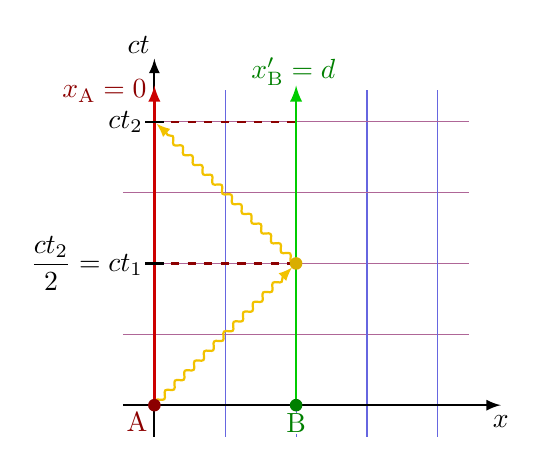
\begin{tikzpicture}[scale=2.0]
  \message{Two observers^^J}
  
  \def\xmin{0.2}
  \def\xmax{2}
  \def\R{2.03} % vector length
  \def\Nlines{4} % number of world lines (at constant x/t)
  \pgfmathsetmacro\d{0.9*\xmax/\Nlines} % grid size
  \pgfmathsetmacro\D{2*\d} % distance between observers
  \coordinate (A) at (0,0); % observer A at t=0
  \coordinate (B) at (\D,0); % observer B at t=0
  \coordinate (C) at (2*\d,2*\d); % point of reflection
  \coordinate (T1) at (0,2*\d); % time of reflection
  \coordinate (T2) at (0,4*\d); % light returning at x=0
  
  % WORLD LINES GRID
  \message{Making world lines...^^J}
  \foreach \i [evaluate={\x=\i*\d;}] in {1,...,\Nlines}{
    \message{  Running i/N=\i/\Nlines, x=\x...^^J}
    \draw[world line]   ( \x,-\xmin) -- ( \x,\xmax);
    \draw[world line t] (-\xmin, \x) -- (\xmax, \x);
  }
  
  % AXES
  \draw[->,thick] (0,-\xmin) -- (0,\xmax+0.2) node[above left=-2] {$ct$};
  \draw[->,thick] (-\xmin,0) -- (\xmax+0.2,0) node[below=0] {$x$};
  \draw[thick,mydarkred,dashed] (T1) -- (C);
  \draw[thick,mydarkred,dashed] (T2) -- (2*\d,4*\d);
  
  % VECTORS
  \draw[vector,myred] (A) --++ (0,\R)
    node[mydarkred,above=-2,left=-1] {\contour{white}{$x_\mathrm{A}=0$}};
  \draw[vector,mygreen] (B) --++ (0,\R)
    node[mydarkgreen,left=1,above=-4] {\contour{white}{$x_\mathrm{B}'=d$}};
  \draw[photon,shorten >=1] (C) -- (T2);
  \fill[mydarkorange] (C) circle(0.04);
  \draw[photon,shorten >=2] (A) -- (C);
  \fill[mydarkred] (A) circle(0.04) node[below left=-1] {A}; % observer A
  \fill[mydarkgreen] (B) circle(0.04) node[fill=white,inner sep=0.5,below=2.5] {B}; % observer B
  
  % TICKS
  \node[fill=white,inner sep=1,left=3] at (T1) {$\dfrac{ct_2}{2}=ct_1$};
  \node[fill=white,inner sep=1,left=3] at (T2) {$ct_2$};
  \tick{T1}{0};
  \tick{T2}{0};
  
\end{tikzpicture}


% SPACETIME DIAGRAM with TWO MOVING OBSERVERS to show simultaneity
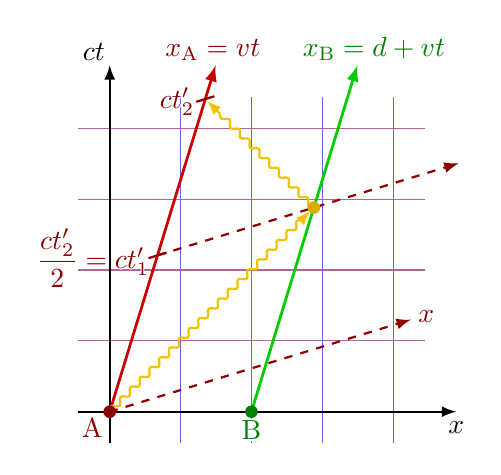
\begin{tikzpicture}[scale=2.0]
  \message{Two moving observers^^J}
  
  \def\xmin{0.2}
  \def\xmax{2}
  \def\R{2.3} % vector length
  \def\Nlines{4} % number of world lines (at constant x/t)
  \pgfmathsetmacro\ang{73} % angle between ct and ct' axes
  \pgfmathsetmacro\d{0.9*\xmax/\Nlines} % grid size
  \pgfmathsetmacro\D{2*\d} % distance between observers
  \coordinate (A) at (0,0); % observer A at t=0
  \coordinate (B) at (\D,0); % observer B at t=0
  \coordinate (C) at (45:{\D*sqrt(2)/(1-cot(\ang))}); % point of reflection
  %\coordinate (T1) at (\ang:{2*\d/sin(\ang)/sqrt(1-cot(\ang)^2)}); % time of reflection
  \coordinate (T1) at (\ang:{\D*sqrt(cot(\ang)^2+1)/(1-cot(\ang)^2)}); % time of reflection
  \coordinate (T2) at (\ang:{2*\D*sqrt(cot(\ang)^2+1)/(1-cot(\ang)^2)}); % time of reflection
  
  % WORLD LINES GRID
  \message{Making world lines...^^J}
  \foreach \i [evaluate={\x=\i*\d;}] in {1,...,\Nlines}{
    \message{  Running i/N=\i/\Nlines, x=\x...^^J}
    \draw[world line]   ( \x,-\xmin) -- ( \x,\xmax);
    \draw[world line t] (-\xmin, \x) -- (\xmax, \x);
  }
  
  % AXES
  \draw[->,thick] (0,-\xmin) -- (0,\xmax+0.2) node[above left=-2] {$ct$};
  \draw[->,thick] (-\xmin,0) -- (\xmax+0.2,0) node[below=0] {$x$};
  \draw[->,thick,mydarkred,dashed] (A) -- (90-\ang:\xmax) node[above=1,right=-1] {$x$}; %_\mathrm{A}'
  \draw[->,thick,mydarkred,dashed] (T1) --++ (90-\ang:\xmax);
  
  % VECTORS
  \draw[vector,myred] (A) --++ (\ang:\R)
    node[mydarkred,left=1,above=-2] {$x_\mathrm{A}=vt$};
  \draw[vector,mygreen] (B) --++ (\ang:\R)
    node[mydarkgreen,right=6,above=-2] {$x_\mathrm{B}=d+vt$};
  \draw[photon,shorten >=1] (C) --++ (135:{\D*sqrt(2)/(1+cot(\ang))});
  \fill[mydarkorange] (C) circle(0.04);
  \draw[photon,shorten >=2] (A) -- (C);
  \fill[mydarkred] (A) circle(0.04) node[below left=-1] {A}; % observer A
  \fill[mydarkgreen] (B) circle(0.04) node[fill=white,inner sep=0.5,below=2.5] {B}; % observer B
  
  % TICKS
  %\node[fill=white,inner sep=1,left=3] at (T1) {$\dfrac{ct_2}{2}=ct_1$};
  %\node[fill=white,inner sep=1,left=3] at (T2) {$ct_2$};
  \tickp{T1}{90-\ang} node[left=-4] {\contour{white}{$\dfrac{ct_2'}{2}=ct_1'$}};
  \tickp{T2}{90-\ang} node[left=-3] {\contour{white}{$ct_2'$}};
  
\end{tikzpicture}


% SPACETIME DIAGRAM of TWIN PARADOX
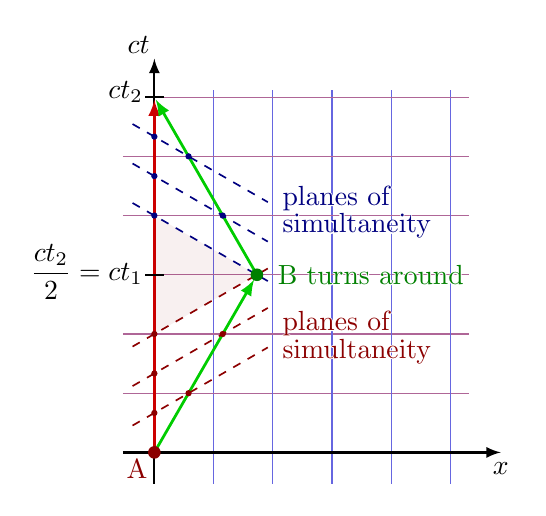
\begin{tikzpicture}[scale=2.0]
  \message{Twin paradox^^J}
  
  \def\xmin{0.2}
  \def\xmax{2}
  \def\ymax{2.3}
  \def\Nlines{5} % number of world lines (at constant x/t)
  \def\ang{60} % angle between ct and ct' axes
  \pgfmathsetmacro\d{0.94*\xmax/\Nlines} % grid size
  \pgfmathsetmacro\dt{3*\d} % time of half trip
  \pgfmathsetmacro\D{\dt/tan(\ang)} % distance between observers
  \pgfmathsetmacro\h{\dt-\D/tan(\ang)} % half time gap of return
  \coordinate (A) at (0,0); % observer A at t=0
  \coordinate (B) at (\D,0); % observer B at t=0
  \coordinate (C) at (\D,\dt); % point of return
  \coordinate (T1) at (0,\dt); % time of return
  \coordinate (T2) at (0,2*\dt); % time of arrival
  
  % WORLD LINES GRID
  \message{Making world lines...^^J}
  \foreach \i [evaluate={\x=\i*\d;}] in {1,...,\Nlines}{
    \message{  Running i/N=\i/\Nlines, x=\x...^^J}
    \draw[world line]   ( \x,-\xmin) -- ( \x,\ymax);
    \draw[world line t] (-\xmin, \x) -- (\xmax, \x);
  }
  \draw[world line t] (-\xmin,{(\Nlines+1)*\d}) -- (\xmax,{(\Nlines+1)*\d});
  
  % AXES
  \draw[->,thick] (0,-\xmin) -- (0,\ymax+0.2) node[above left=-2] {$ct$};
  \draw[->,thick] (-\xmin,0) -- (\xmax+0.2,0) node[below=0] {$x$};
  
  % VECTORS
  \draw[vector,myred,shorten >=1] (A) -- (T2);
  \draw[vector,mygreen,shorten >=2] (A) -- (C);
  \draw[vector,mygreen,shorten >=1] (C) -- (T2);
  
  % PLANES OF SIMULTANEITY
  \fill[mydarkred,opacity=0.06]
    (0,\h) -- (C) -- (0,2*\dt-\h) -- cycle;
  \pgfmathsetmacro\ystep{\h/3}
  \foreach \i [evaluate={\dy=(\i-1)*\ystep; \ya=\i*\ystep; \yb=2*\dt-\i*\ystep;}] in {1,...,3}{
    \draw[mydarkred,dashed,line width=0.6]
      (0,\ya)++(90-\ang:-0.8*\xmin) --++ (90-\ang:{1.2*\xmin+\D/sin(\ang)});
    \draw[mydarkblue,dashed,line width=0.6]
      (0,\yb)++(\ang-90:-0.8*\xmin) --++ (\ang-90:{1.2*\xmin+\D/sin(\ang)});
    \fill[mydarkred]  (0,\ya) circle(0.02);
    \fill[mydarkblue] (0,\yb) circle(0.02);
    %\fill[mydarkblue] ({\D-\dy*cot(\ang)},\dt+\dy) circle(0.02);
    %\fill[mydarkred]  ({\D-\dy*cot(\ang)},\dt-\dy) circle(0.02);
    \fill[mydarkblue] (C)++(-\ang:{\dy*sin(\ang)/cos(2*\ang)}) circle(0.02);
    \fill[mydarkred]  (C)++( \ang:{\dy*sin(\ang)/cos(2*\ang)}) circle(0.02);
  }
  \fill[mydarkred] (A) circle(0.04) node[below left=-1] {A}; % observer A
  \fill[mydarkgreen] (C) circle(0.04)
    node[right=4] {\contour{white}{B turns around}}; % observer B returns
  \node[mydarkblue,above right=0,align=left] at (2*\d,1.15*\dt)
    {\contour{white}{planes of}\\[-2]\contour{white}{simultaneity}};
  \node[mydarkred,below right=0,align=left] at (2*\d,0.85*\dt)
    {\contour{white}{planes of}\\[-2]\contour{white}{simultaneity}};
  
  % TICKS
  \node[fill=white,inner sep=1,above=1,left=3] at (T1) {$\dfrac{ct_2}{2}=ct_1$};
  \node[fill=white,inner sep=1,above=2,left=3] at (T2) {$ct_2$};
  \tick{T1}{0};
  \tick{T2}{0};
  
\end{tikzpicture}


% SPACETIME DIAGRAM - GALILEAN TRANSFORMATION
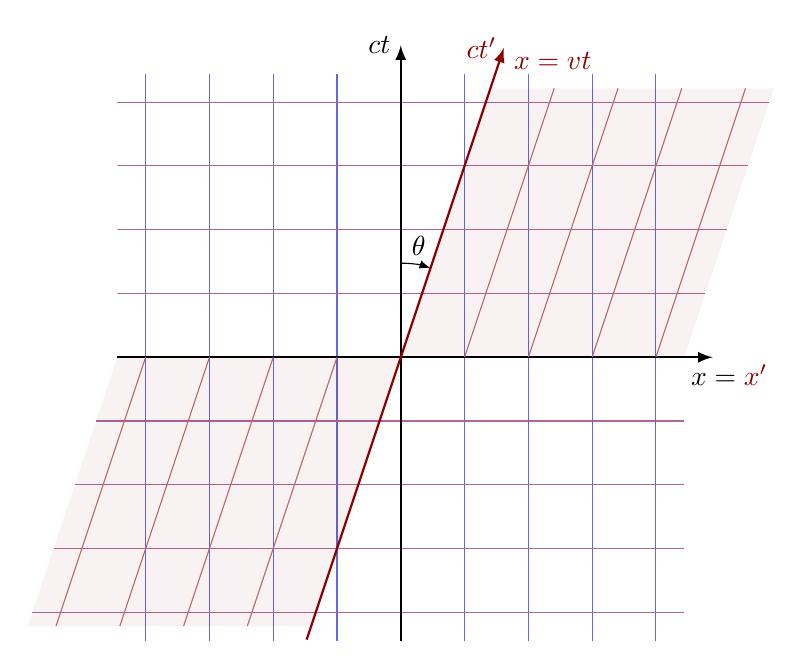
\begin{tikzpicture}[scale=1.8]
  \message{Galilean transformation^^J}
  
  \def\xmax{2}
  \def\xmaxp{2.1} % maximum of rotated axis
  \def\Nlines{4} % number of world lines (at constant x/t)
  \pgfmathsetmacro\d{0.9*\xmax/\Nlines} % grid size
  \pgfmathsetmacro\ang{atan(1/3)} % angle
  \coordinate (O) at (0,0);
  \coordinate (X) at (\xmax+0.2,0);
  \coordinate (T) at (0,\xmax+0.2);
  \coordinate (X') at (\ang:\xmaxp+0.2);
  \coordinate (T') at (90-\ang:\xmaxp+0.2);
  
  % WORLD LINES GRID
  \message{Making world lines...^^J}
  \foreach \i [evaluate={\x=\i*\d;}] in {1,...,\Nlines}{
    \message{  Running i/N=\i/\Nlines, x=\x...^^J}
    \draw[world line]   (-\x,-\xmax) -- (-\x,\xmax);
    \draw[world line]   ( \x,-\xmax) -- ( \x,\xmax);
    \draw[world line t] ({-\xmax-tan(\ang)*\x},-\x) -- (\xmax,-\x);
    \draw[world line t] (-\xmax,\x) -- ({\xmax+tan(\ang)*\x},\x);
  }
  
  % AXES
  \draw[->,thick] (0,-\xmax) -- (T) node[left=0] {$ct$};
  \draw[->,thick] (-\xmax,0) -- (X) node[right=6,below=-1] {$x={\color{mydarkred}x'}$};
  \draw[->,thick,mydarkred] (90-\ang:-\xmaxp) -- (T')
    node[left=-1] {$ct'$}
    node[right=2,below right=-2] {$x = vt$};
  
  % WORLD LINES GRID - BOOSTED
  \message{Making world lines, boosted...^^J}
  \fill[mydarkred,opacity=0.05]
    (O) --++ (90-\ang:\xmax) --++ (\xmax,0) --++ (90-\ang:-\xmax) -- cycle;
  \fill[mydarkred,opacity=0.05]
    (O) --++ (90-\ang:-\xmax) --++ (-\xmax,0) --++ (90-\ang:\xmax) -- cycle;
  \foreach \i [evaluate={\x=\i*\d;}] in {1,...,\Nlines}{
    \message{  Running i/N=\i/\Nlines, x=\x...^^J}
    \draw[world line'] (\x,0) --++ (90-\ang:\xmax);
    \draw[world line'] (-\x,0) --++ (90-\ang:-\xmax);
  }
  
  \draw pic[<-,"$\theta$",draw=black,angle radius=34,angle eccentricity=1.2] {angle = T'--O--T};
  
\end{tikzpicture}


% SPACETIME DIAGRAM - LIGHT CONE
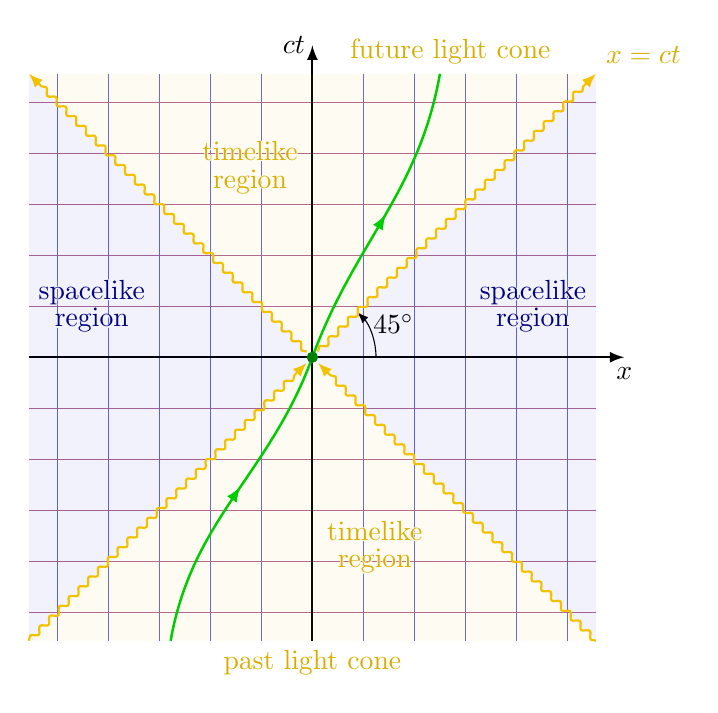
\begin{tikzpicture}[scale=1.8]
  \message{Light cone^^J}
  
  \def\xmax{2}
  \def\xmaxp{2.2} % maximum of rotated axis
  \def\Nlines{5} % number of world lines (at constant x/t)
  \pgfmathsetmacro\d{0.9*\xmax/\Nlines} % grid size
  \pgfmathsetmacro\ang{atan(1/3)} % angle between x and x' axes
  \coordinate (O) at (0,0);
  \coordinate (X) at (\xmax+0.2,0);
  \coordinate (T) at (0,\xmax+0.2);
  \coordinate (C) at (45:\xmaxp+0.2);
  \coordinate (E) at (4*\d,0); % event
  
  % WORLD LINE GRID
  \message{Making world lines...^^J}
  \foreach \i [evaluate={\x=\i*\d;}] in {1,...,\Nlines}{
    \message{  Running i/N=\i/\Nlines, x=\x...^^J}
    \draw[world line]   (-\x,-\xmax) -- (-\x,\xmax);
    \draw[world line]   ( \x,-\xmax) -- ( \x,\xmax);
    \draw[world line t] (-\xmax,-\x) -- (\xmax,-\x);
    \draw[world line t] (-\xmax, \x) -- (\xmax, \x);
  }
  
  % AXES
  \draw[->,thick] (0,-\xmax) -- (T) node[left=-1] {$ct$};
  \draw[->,thick] (-\xmax,0) -- (X) node[below=0] {$x$};
  
  % LABELS
  \draw pic[->,"$45^\circ$",draw=black,angle radius=23,angle eccentricity=1.38] {angle = X--O--C};
  \node[mydarkorange,above right] at (0.1*\xmax,\xmax) {future light cone};
  \node[mydarkorange,below] at (0,-\xmax) {past light cone};
  
  % FILLS
  \fill[myblue,opacity=0.05] % SPACELIKE
    (\xmax,\xmax) -- (-\xmax,-\xmax) -- (-\xmax,\xmax) -- (\xmax,-\xmax) -- cycle;
  \fill[myorange,opacity=0.05] % TIMELIKE
    (\xmax,\xmax) -- (-\xmax,\xmax) -- (\xmax,-\xmax) -- (-\xmax,-\xmax) -- cycle;
  \node[mydarkblue,right,align=center] at (-\xmax,0.18*\xmax)
    {\contour{myblue!5}{spacelike}\\[-2]\contour{myblue!5}{region}};
  \node[mydarkblue,left,align=center] at (\xmax,0.18*\xmax)
    {\contour{myblue!5}{spacelike}\\[-2]\contour{myblue!5}{region}};
  \node[mydarkorange,align=center] at (-0.22*\xmax,0.67*\xmax)
    {\contour{myorange!5}{timelike}\\[-2]\contour{myorange!5}{region}};
  \node[mydarkorange,align=center] at (0.22*\xmax,-0.67*\xmax)
    {\contour{myorange!5}{timelike}\\[-2]\contour{myorange!5}{region}};
  
  % PHOTON
  \draw[photon] ( \xmax,-\xmax) -- ( 0.02*\xmax,-0.02*\xmax);
  \draw[photon] (-\xmax,-\xmax) -- (-0.02*\xmax,-0.02*\xmax);
  \draw[photon] ( 0.02*\xmax,0.02*\xmax) -- ( \xmax,\xmax)
    node[mydarkorange,above right] {$x=ct$};
  \draw[photon] (-0.02*\xmax,0.02*\xmax) -- (-\xmax,\xmax);
  
  % PARTICLE WORLDLINE
  \draw[particle,decoration={markings,mark=at position 0.27 with {\arrow{latex}},
                                      mark=at position 0.76 with {\arrow{latex}}},postaction={decorate}]
      (-0.5*\xmax,-\xmax) to[out=80,in=-110] (O) to[out=70,in=-100] (0.45*\xmax,\xmax);
  \fill[mydarkgreen] (O) circle(0.04); % event
  
\end{tikzpicture}


% SPACETIME DIAGRAM - VECTORS
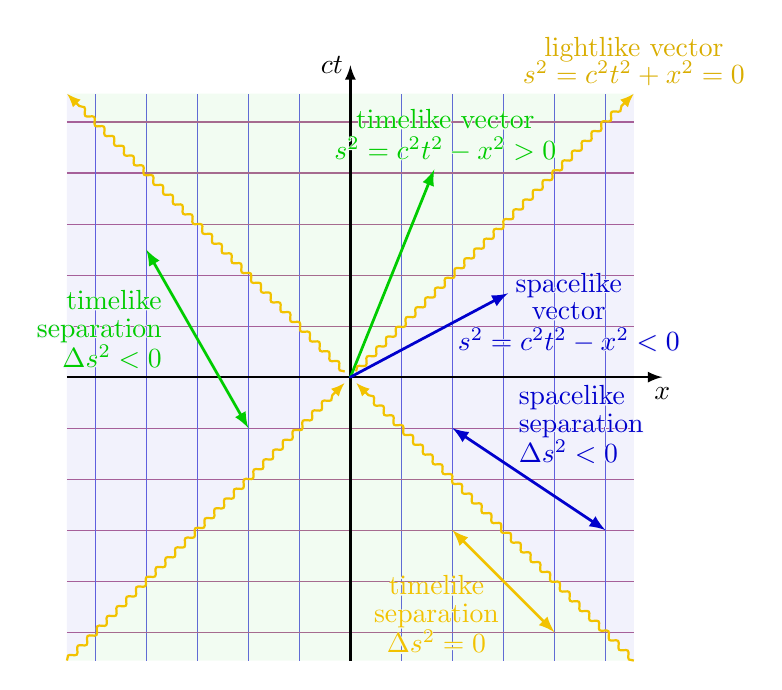
\begin{tikzpicture}[scale=1.8]
  \message{Vectors^^J}
  
  \def\xmax{2}
  \def\xmaxp{2.2} % maximum of rotated axis
  \def\Nlines{5} % number of world lines (at constant x/t)
  \pgfmathsetmacro\d{0.9*\xmax/\Nlines} % grid size
  \pgfmathsetmacro\ang{atan(1/3)} % angle between x and x' axes
  \coordinate (O) at (0,0);
  \coordinate (X) at (\xmax+0.2,0);
  \coordinate (T) at (0,\xmax+0.2);
  \coordinate (C) at (45:\xmaxp+0.2);
  \coordinate (E) at (4*\d,0); % event
  
  % WORLD LINE GRID
  \message{Making world lines...^^J}
  \foreach \i [evaluate={\x=\i*\d;}] in {1,...,\Nlines}{
    \message{  Running i/N=\i/\Nlines, x=\x...^^J}
    \draw[world line]   (-\x,-\xmax) -- (-\x,\xmax);
    \draw[world line]   ( \x,-\xmax) -- ( \x,\xmax);
    \draw[world line t] (-\xmax,-\x) -- (\xmax,-\x);
    \draw[world line t] (-\xmax, \x) -- (\xmax, \x);
  }
  
  % FILLS
  \fill[myblue,opacity=0.05] % SPACELIKE
    (\xmax,\xmax) -- (-\xmax,-\xmax) -- (-\xmax,\xmax) -- (\xmax,-\xmax) -- cycle;
  \fill[mygreen,opacity=0.05] % TIMELIKE
    (\xmax,\xmax) -- (-\xmax,\xmax) -- (\xmax,-\xmax) -- (-\xmax,-\xmax) -- cycle;
  
  % AXES
  \draw[->,thick] (0,-\xmax) -- (T) node[left=-1] {$ct$};
  \draw[->,thick] (-\xmax,0) -- (X) node[below=0] {$x$};
  
  % VECTORS
  \draw[vector,mygreen] (O) --++ (68:0.79*\xmax)
    node[right=4,above=-1,align=center]
    {\contour{mygreen!5}{timelike vector}\\[-1]
     \contour{mygreen!5}{$s^2=c^2t^2-x^2>0$}};
  \draw[vector,myblue] (O) --++ (28:0.63*\xmax)
    node[below=7,right=-22,align=center]
    {\contour{myblue!5}{spacelike}\\[-2]
     \contour{myblue!5}{vector}\\[-1]
     \contour{myblue!5}{$s^2=c^2t^2-x^2<0$}};
  \draw[vector,mygreen,<->] (-2*\d,-\d) --++ (-2*\d,3.5*\d)
    node[pos=0.8,below left=-2,align=right]
    {\contour{myblue!5}{timelike}\\[-2]
     \contour{myblue!5}{separation}\\[-1]
     \contour{myblue!5}{$\Delta s^2<0$}};
  \draw[vector,myblue,<->] (2*\d,-\d) --++ (3*\d,-2*\d)
    node[pos=0.4,above right=-2,align=left]
    {\contour{myblue!5}{spacelike}\\[-2]
     \contour{myblue!5}{separation}\\[-1]
     \contour{myblue!5}{$\Delta s^2<0$}};
  \draw[vector,myorange,<->] (2*\d,-3*\d) --++ (2*\d,-2*\d)
    node[pos=0.45,below left=-4,align=center]
    {\contour{mygreen!5}{timelike}\\[-2]
     \contour{mygreen!5}{separation}\\[-1]
     \contour{mygreen!5}{$\Delta s^2 = 0$}};
  
  % PHOTON
  \draw[photon] ( \xmax,-\xmax) -- ( 0.02*\xmax,-0.02*\xmax);
  \draw[photon] (-\xmax,-\xmax) -- (-0.02*\xmax,-0.02*\xmax);
  \draw[photon] ( 0.02*\xmax,0.02*\xmax) -- ( \xmax,\xmax)
    node[mydarkorange,above=-1,align=center] {lightlike vector\\[-2]$s^2=c^2t^2+x^2=0$};
  \draw[photon] (-0.02*\xmax,0.02*\xmax) -- (-\xmax,\xmax);
  
\end{tikzpicture}


% SPACETIME DIAGRAM - OVERLAPPING LIGHT CONES
\begin{tikzpicture}[scale=1.8]
  \message{Overlapping light cones^^J}
  
  \def\xmax{2}
  \def\ext{4*\d} % extension
  \def\xmaxp{2.2} % maximum of rotated axis
  \def\Nlines{5} % number of world lines (at constant x/t)
  \pgfmathsetmacro\d{0.9*\xmax/\Nlines} % grid size
  \pgfmathsetmacro\ang{atan(1/3)} % angle between x and x' axes
  \coordinate (O) at (0,0);
  \coordinate (X) at (\xmax+\ext+0.2,0);
  \coordinate (T) at (0,\xmax+0.2);
  \coordinate (C) at (45:\xmaxp+0.2);
  \coordinate (B) at (4*\d,0); % event B
  
  % WORLD LINE GRID
  \message{Making world lines...^^J}
  \foreach \i [evaluate={\x=\i*\d;}] in {1,...,\Nlines}{
    \message{  Running i/N=\i/\Nlines, x=\x...^^J}
    \draw[world line]   (-\x,-\xmax) -- (-\x,\xmax);
    \draw[world line]   ( \x,-\xmax) -- ( \x,\xmax);
    \draw[world line t] (-\xmax,-\x) -- (\xmax+\ext,-\x);
    \draw[world line t] (-\xmax, \x) -- (\xmax+\ext, \x);
  }
  \foreach \i [evaluate={\x=(\Nlines+\i)*\d;}] in {1,...,4}{
    \message{  Running i/N=\i/\Nlines, x=\x...^^J}
    \draw[world line] (\x,-\xmax) -- ( \x,\xmax);
  }
  
  % AXES
  \draw[->,thick] (0,-\xmax) -- (T) node[left=-1] {${\color{mydarkred}ct'}=ct$};
  \draw[->,thick] (-\xmax,0) -- (X) node[below=0] {$x$};
  
  % PHOTON
  \begin{scope}[shift={(E)}]
    \fill[myorange!70!red,opacity=0.07]
      (0,0) -- (\xmax,\xmax) -- (-\xmax,\xmax) -- (\xmax,-\xmax) -- (-\xmax,-\xmax) -- cycle;
  \end{scope}
  \fill[myorange!70!green,opacity=0.07]
    (O) -- (\xmax,\xmax) -- (-\xmax,\xmax) -- (\xmax,-\xmax) -- (-\xmax,-\xmax) -- cycle;
  \draw[photon] (-0.05,0.05) -- (135:0.4*\xmax);
  \draw[photon] (0.05,0.05) -- (45:0.4*\xmax);
  %\draw[photon] (0.05,0.05) -- ( \xmax,\xmax)
  %  node[mydarkorange,above right] {$x=ct$};
  \draw[photon] (E)++(-0.05,0.05) --++ (135:0.4*\xmax);
  \draw[photon] (E)++(0.05,0.05) --++ (45:0.4*\xmax);
  
  % PARTICLE WORLDLINES
  \draw[particle,decoration={markings,mark=at position 0.27 with {\arrow{latex}},
                                      mark=at position 0.76 with {\arrow{latex}}},postaction={decorate}]
      (-0.5*\xmax,-\xmax) to[out=80,in=-110] (O) to[out=70,in=-100] (0.45*\xmax,\xmax);
  \draw[particle,myred,decoration={markings,mark=at position 0.27 with {\arrow{latex}},
                                            mark=at position 0.74 with {\arrow{latex}}},postaction={decorate}]
      (0.84*\xmax,-\xmax) to[out=95,in=-80] (E) to[out=100,in=-76] (0.49*\xmax,\xmax);
  \fill[mydarkgreen] (O) circle(0.04); % event A
  \fill[mydarkred] (B) circle(0.04); % event B
  
\end{tikzpicture}


% SPACETIME DIAGRAM - LORENTZ BOOST
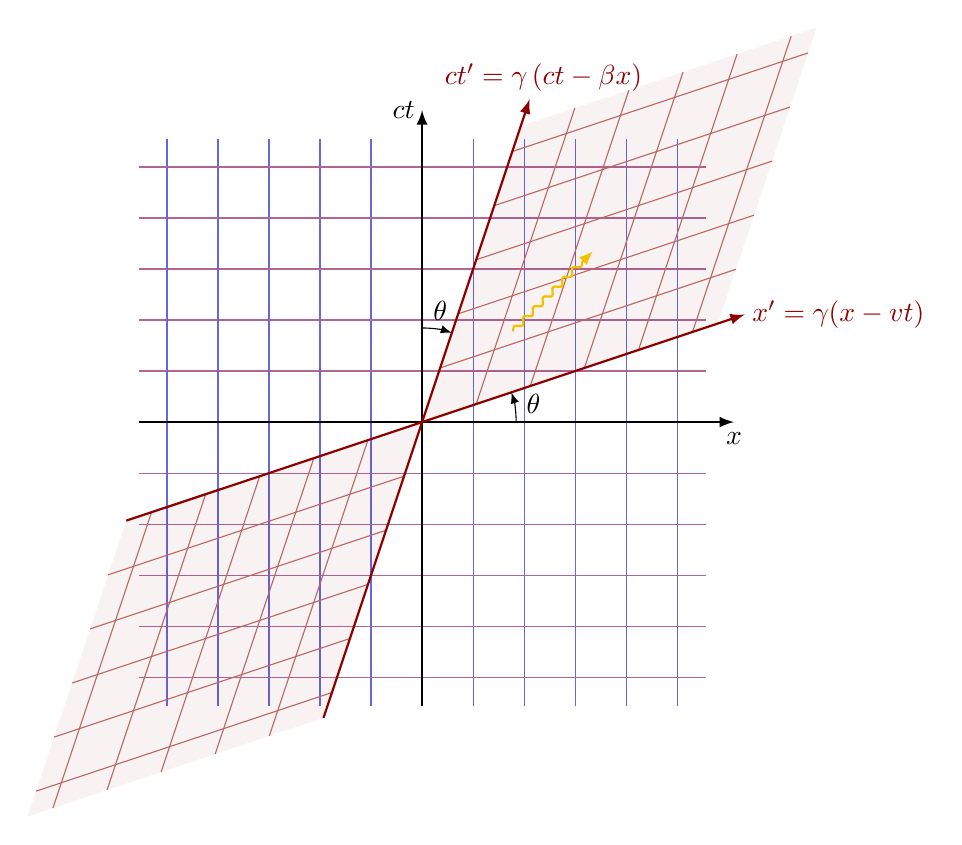
\begin{tikzpicture}[scale=1.8]
  \message{Lorentz boost^^J}
  
  \def\xmax{2}
  \def\xmaxp{2.2} % maximum of rotated axis
  \def\Nlines{5} % number of world lines (at constant x/t)
  \pgfmathsetmacro\ang{atan(1/3)} % angle between x and x' axes
  \pgfmathsetmacro\d{0.9*\xmax/\Nlines} % grid size
  \pgfmathsetmacro\D{\d/cos(\ang)/sqrt(1-tan(\ang)^2)} % grid size, boosted
  \coordinate (O) at (0,0);
  \coordinate (X) at (\xmax+0.2,0);
  \coordinate (T) at (0,\xmax+0.2);
  \coordinate (X') at (\ang:\xmaxp+0.2);
  \coordinate (T') at (90-\ang:\xmaxp+0.2);
  
  % WORLD LINE GRID
  \message{Making world lines...^^J}
  \foreach \i [evaluate={\x=\i*\d;}] in {1,...,\Nlines}{
    \message{  Running i/N=\i/\Nlines, x=\x...^^J}
    \draw[world line]   (-\x,-\xmax) -- (-\x,\xmax);
    \draw[world line]   ( \x,-\xmax) -- ( \x,\xmax);
    \draw[world line t] (-\xmax,-\x) -- (\xmax,-\x);
    \draw[world line t] (-\xmax, \x) -- (\xmax, \x);
  }
  
  % BOOSTED WORLD LINE GRID
  \message{Making world lines for boosted frame...^^J}
  \fill[mydarkred,opacity=0.05]
    (O) --++ (\ang:\xmaxp) --++ (90-\ang:\xmaxp) --++ (\ang:-\xmaxp) -- cycle;
  \fill[mydarkred,opacity=0.05]
    (O) --++ (\ang:-\xmaxp) --++ (90-\ang:-\xmaxp) --++ (\ang:\xmaxp) -- cycle;
  \foreach \i [evaluate={\x=\i*\D;}] in {1,...,\Nlines}{
    \message{  Running i/N=\i/\Nlines, x=\x...^^J}
    \draw[world line'] (\ang:-\x) --++ (90-\ang:-\xmaxp);
    \draw[world line'] (90-\ang:-\x) --++ (\ang:-\xmaxp);
    \draw[world line'] (\ang:\x) --++ (90-\ang:\xmaxp);
    \draw[world line'] (90-\ang:\x) --++ (\ang:\xmaxp);
  }
  
  % AXES
  \draw[->,thick] (0,-\xmax) -- (T) node[left=-1] {$ct$};
  \draw[->,thick] (-\xmax,0) -- (X) node[below=0] {$x$};
  \draw[->,thick,mydarkred] (90-\ang:-\xmaxp) -- (T')
    node[right=5,above=-1] {$ct' = \gamma\left(ct-\beta x\right)$};
  \draw[->,thick,mydarkred] (\ang:-\xmaxp) -- (X') node[right=-1] {$x' = \gamma(x-vt)$};
  
  % ANGLES
  \draw pic[->,"$\theta$",draw=black,angle radius=34,angle eccentricity=1.2] {angle = X--O--X'};
  \draw pic[<-,"$\theta$",draw=black,angle radius=34,angle eccentricity=1.2] {angle = T'--O--T};
  
  % PHOTON
  \draw[photon] (0.32*\xmax,0.32*\xmax) --++ (45:0.4*\xmax);
  
\end{tikzpicture}


% SPACETIME DIAGRAM - INVERSE LORENTZ BOOST
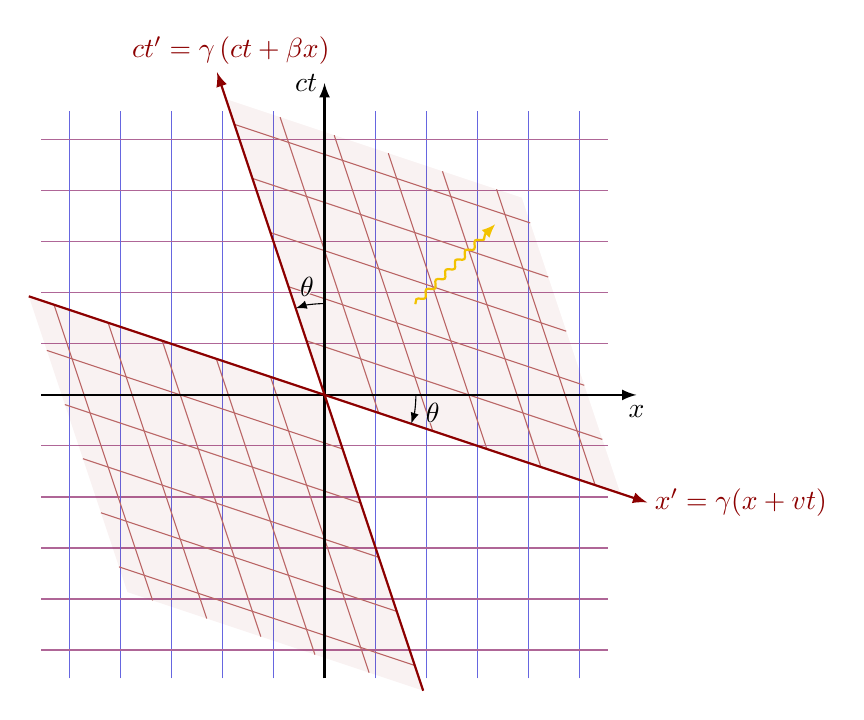
\begin{tikzpicture}[scale=1.8]
  \message{Inverse Lorentz boost^^J}
  
  \def\xmax{2}
  \def\xmaxp{2.2} % maximum of rotated axis
  \def\Nlines{5} % number of world lines (at constant x/t)
  \pgfmathsetmacro\ang{atan(-1/3)} % inverted angle
  \pgfmathsetmacro\d{0.9*\xmax/\Nlines} % grid size
  \pgfmathsetmacro\D{\d/cos(\ang)/sqrt(1-tan(\ang)^2)} % grid size, boosted
  \coordinate (O) at (0,0);
  \coordinate (X) at (\xmax+0.2,0);
  \coordinate (T) at (0,\xmax+0.2);
  \coordinate (X') at (\ang:\xmaxp+0.2);
  \coordinate (T') at (90-\ang:\xmaxp+0.2);
  
  % WORLD LINE GRID
  \message{Making world lines...^^J}
  \foreach \i [evaluate={\x=\i*\d;}] in {1,...,\Nlines}{
    \message{  Running i/N=\i/\Nlines, x=\x...^^J}
    \draw[world line]   (-\x,-\xmax) -- (-\x,\xmax);
    \draw[world line]   ( \x,-\xmax) -- ( \x,\xmax);
    \draw[world line t] (-\xmax,-\x) -- (\xmax,-\x);
    \draw[world line t] (-\xmax, \x) -- (\xmax, \x);
  }
  
  % BOOSTED WORLD LINE GRID
  \message{Making world lines for boosted frame...^^J}
  \fill[mydarkred,opacity=0.05]
    (O) --++ (\ang:\xmaxp) --++ (90-\ang:\xmaxp) --++ (\ang:-\xmaxp) -- cycle;
  \fill[mydarkred,opacity=0.05]
    (O) --++ (\ang:-\xmaxp) --++ (90-\ang:-\xmaxp) --++ (\ang:\xmaxp) -- cycle;
  \foreach \i [evaluate={\x=\i*\D;}] in {1,...,\Nlines}{
    \message{  Running i/N=\i/\Nlines, x=\x...^^J}
    \draw[world line'] (\ang:-\x) --++ (90-\ang:-\xmaxp);
    \draw[world line'] (90-\ang:-\x) --++ (\ang:-\xmaxp);
    \draw[world line'] (\ang:\x) --++ (90-\ang:\xmaxp);
    \draw[world line'] (90-\ang:\x) --++ (\ang:\xmaxp);
  }
  
  % AXES
  \draw[->,thick] (0,-\xmax) -- (T) node[left=-1] {$ct$};
  \draw[->,thick] (-\xmax,0) -- (X) node[below=0] {$x$};
  \draw[->,thick,mydarkred] (90-\ang:-\xmaxp) -- (T')
    node[right=5,above=-1] {$ct' = \gamma\left(ct+\beta x\right)$};
  \draw[->,thick,mydarkred] (\ang:-\xmaxp) -- (X') node[right=-1] {$x' = \gamma(x+vt)$};
  
  % ANGLES
  \draw pic[<-,"\contour{mydarkred!5}{$\theta$}",draw=black,angle radius=33,angle eccentricity=1.2] {angle = X'--O--X};
  \draw pic[->,"\contour{mydarkred!5}{$\theta$}",draw=black,angle radius=33,angle eccentricity=1.2] {angle = T--O--T'};
  
  % PHOTON
  \draw[photon] (0.32*\xmax,0.32*\xmax) --++ (45:0.4*\xmax);
  
\end{tikzpicture}


% SPACETIME DIAGRAM - ROTATION
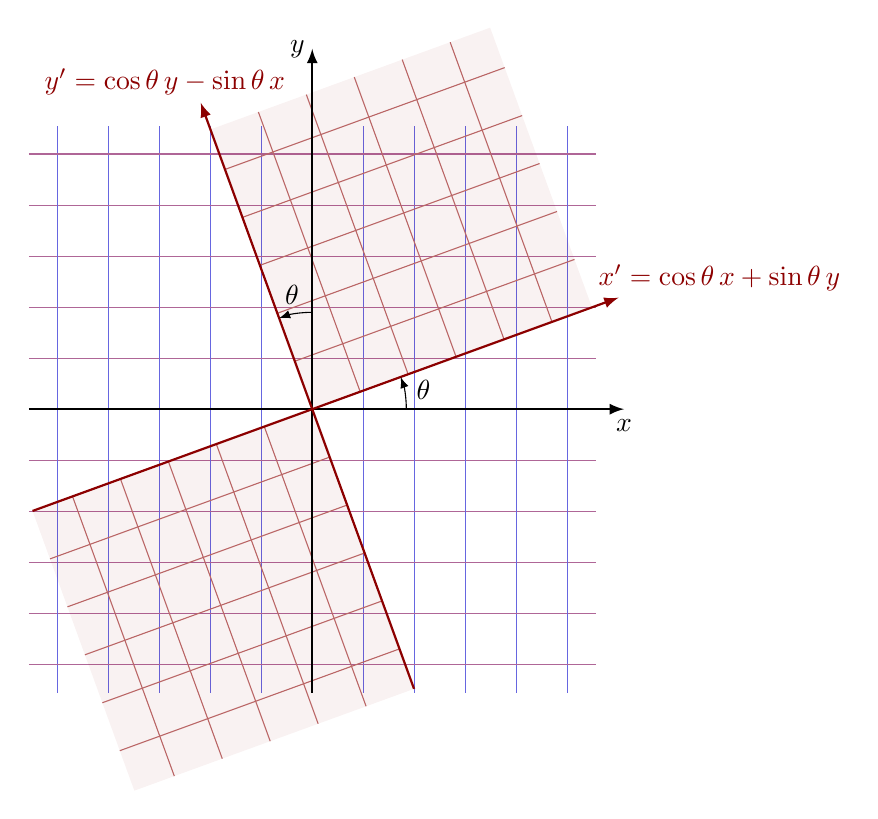
\begin{tikzpicture}[scale=1.8]
  \message{Rotation^^J}
  
  \def\xmax{2}
  \def\xmaxp{2.1} % maximum of rotated axis
  \def\Nlines{5} % number of world lines (at constant x/t)
  \pgfmathsetmacro\ang{20} % angle between x and x' axes
  \pgfmathsetmacro\d{0.9*\xmax/\Nlines} % grid size
  \coordinate (O) at (0,0);
  \coordinate (X) at (\xmax+0.2,0);
  \coordinate (T) at (0,{(1+0.5*sin(\ang))*\xmax+0.2});
  \coordinate (X') at (\ang:\xmaxp+0.2);
  \coordinate (T') at (90+\ang:\xmaxp+0.2);
  
  % WORLD LINE GRID
  \message{Making world lines...^^J}
  \foreach \i [evaluate={\x=\i*\d;}] in {1,...,\Nlines}{
    \message{  Running i/N=\i/\Nlines, x=\x...^^J}
    \draw[world line]   (-\x,-\xmax) -- (-\x,\xmax);
    \draw[world line]   ( \x,-\xmax) -- ( \x,\xmax);
    \draw[world line t] (-\xmax,-\x) -- (\xmax,-\x);
    \draw[world line t] (-\xmax, \x) -- (\xmax, \x);
  }
  
  % BOOSTED WORLD LINE GRID
  \message{Making world lines for boosted frame...^^J}
  \fill[mydarkred,opacity=0.05]
    (O) --++ (\ang:\xmaxp) --++ (90+\ang:\xmaxp) --++ (\ang:-\xmaxp) -- cycle;
  \fill[mydarkred,opacity=0.05]
    (O) --++ (\ang:-\xmaxp) --++ (90+\ang:-\xmaxp) --++ (\ang:\xmaxp) -- cycle;
  \foreach \i [evaluate={\x=\i*\d;}] in {1,...,\Nlines}{
    \message{  Running i/N=\i/\Nlines, x=\x...^^J}
    \draw[world line'] (\ang:-\x) --++ (90+\ang:-\xmaxp);
    \draw[world line'] (90+\ang:-\x) --++ (\ang:-\xmaxp);
    \draw[world line'] (\ang:\x) --++ (90+\ang:\xmaxp);
    \draw[world line'] (90+\ang:\x) --++ (\ang:\xmaxp);
  }
  
  % AXES
  \draw[->,thick] (0,-\xmax) -- (T) node[left=-1] {$y$};
  \draw[->,thick] (-\xmax,0) -- (X) node[below=0] {$x$};
  \draw[->,thick,mydarkred] (90+\ang:-\xmaxp) -- (T')
    node[left=13,above=-1] {$y'=\cos\theta\,y-\sin\theta\,x$};
  \draw[->,thick,mydarkred] (\ang:-\xmaxp) -- (X')
    node[above=7,right=-11] {$x'=\cos\theta\,x+\sin\theta\,y$};
  
  % ANGLES
  \draw pic[->,"$\theta$",draw=black,angle radius=34,angle eccentricity=1.2] {angle = X--O--X'};
  \draw pic[->,"$\theta$",draw=black,angle radius=35,angle eccentricity=1.2] {angle = T--O--T'};
  
\end{tikzpicture}


% SPACETIME DIAGRAM - SIMULTANEITY
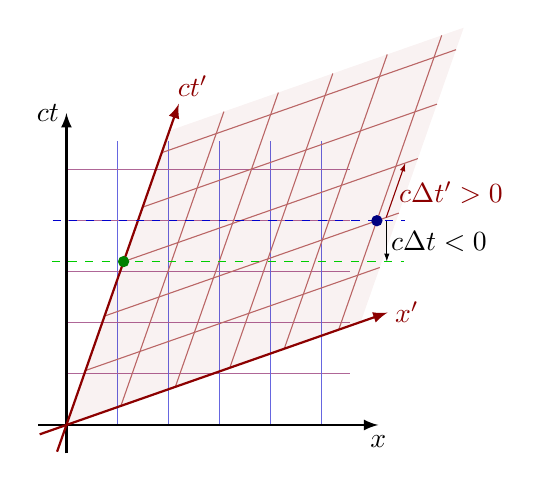
\begin{tikzpicture}[scale=1.8]
  \message{Simultaneity^^J}
  
  \def\xmin{0.2}
  \def\xmax{2}
  \def\xmaxp{2.2} % maximum of rotated axis
  \def\Nlines{5} % number of world lines (at constant x/t)
  \pgfmathsetmacro\ang{atan(0.35)} % angle between x and x' axes
  \pgfmathsetmacro\d{0.9*\xmax/\Nlines} % grid size
  \pgfmathsetmacro\D{\d/cos(\ang)/sqrt(1-tan(\ang)^2)} % grid size, boosted
  \coordinate (O) at (0,0);
  \coordinate (X) at (\xmax+0.2,0);
  \coordinate (T) at (0,\xmax+0.2);
  \coordinate (X') at (\ang:\xmaxp+0.2);
  \coordinate (T') at (90-\ang:\xmaxp+0.2);
  
  % WORLD LINE GRID
  \message{Making world lines...^^J}
  \foreach \i [evaluate={\x=\i*\d;}] in {1,...,\Nlines}{
    \message{  Running i/N=\i/\Nlines, x=\x...^^J}
    \draw[world line]   (\x,0) -- ( \x,\xmax);
    \draw[world line t] (0,\x) -- (\xmax, \x);
  }
  
  % BOOSTED WORLD LINE GRID
  \message{Making world lines for boosted frame...^^J}
  \fill[mydarkred,opacity=0.05]
    (O) --++ (\ang:\xmaxp) --++ (90-\ang:\xmaxp) --++ (\ang:-\xmaxp) -- cycle;
  \foreach \i [evaluate={\x=\i*\D;}] in {1,...,\Nlines}{
    \message{  Running i/N=\i/\Nlines, x=\x...^^J}
    \draw[world line'] (\ang:\x) --++ (90-\ang:\xmaxp);
    \draw[world line'] (90-\ang:\x) --++ (\ang:\xmaxp);
  }
  
  % AXES
  \draw[->,thick] (0,-\xmin) -- (T) node[left=-1] {$ct$};
  \draw[->,thick] (-\xmin,0) -- (X) node[below=0] {$x$};
  \draw[->,thick,mydarkred] (90-\ang:-\xmin) -- (T')
    node[right=5,above=-1] {$ct'$};
  \draw[->,thick,mydarkred] (\ang:-\xmin) -- (X') node[right=-1] {$x'$};
  
  % EVENTS
  \draw[mygreen,mydashed,thin]
    (90-\ang:3*\D) coordinate (A) ++ (-0.23*\xmaxp,0) --++ (1.13*\xmaxp,0);
  \draw[myblue,mydashed,thin]
    (\ang:5*\D)++(90-\ang:2*\D) coordinate (B)++(-1.04*\xmaxp,0) --++ (1.13*\xmaxp,0);
  \draw[mysmallarr,mydarkred] (B)++(\ang:0.07) --++ (90-\ang:\D)
    node[pos=0.46,right=-2] {$c\Delta t'>0$};
  \draw[mysmallarr] (B)++(0.07,0) --++ (0,-0.29)
    node[pos=0.5,right=-2] {$c\Delta t<0$};
  \fill[mydarkgreen] (A) circle(0.04); % event A
  \fill[mydarkblue] (B) circle(0.04); % event B
  
\end{tikzpicture}


% SPACETIME DIAGRAM - INVARIANT HYPERBOLOIDS
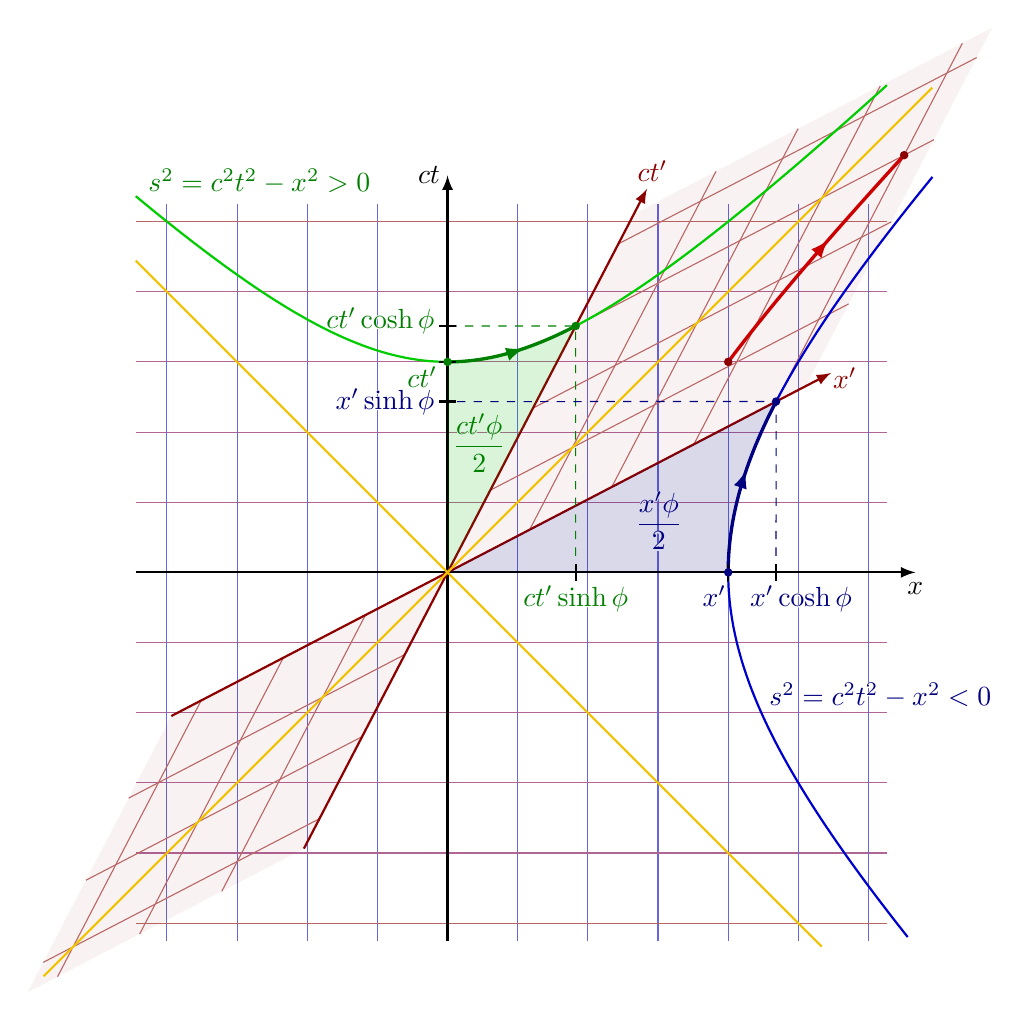
\begin{tikzpicture}[scale=1.8]
  \message{Invariant hyperboloids^^J}
  
  \def\xmin{2.2}
  \def\xmax{3.1}
  \def\ymax{2.6}
  \def\xmaxp{2.85} % maximum of rotated axis
  \def\Nlines{4} % number of world lines (at constant x/t)
  \pgfmathsetmacro\ang{atan(0.52)} % angle between x and x' axes
  \pgfmathsetmacro\d{0.9*\xmin/\Nlines} % grid size
  \pgfmathsetmacro\D{\d/cos(\ang)/sqrt(1-tan(\ang)^2)} % grid size, boosted
  \pgfmathsetmacro\dextra{(\Nlines+1)*\d} % extra line
  \pgfmathsetmacro\st{3*\d} % spacetime interval
  \pgfmathsetmacro\sx{4*\d} % spacetime interval
  \pgfmathsetmacro\sr{sqrt(\sx^2-\st^2)} % spacetime interval sr^2 = st^2 - sx^2 < 0
  \pgfmathsetmacro\Ax{3*\D*sin(\ang)} % x coordinate of event A
  \pgfmathsetmacro\Ay{3*\D*cos(\ang)} % y coordinate of event A
  \pgfmathsetmacro\Bx{4*\D*cos(\ang)} % x coordinate of event B
  \pgfmathsetmacro\By{4*\D*sin(\ang)} % y coordinate of event B
  \pgfmathsetmacro\Cx{\Ay+\By} % x coordinate of event C' %(\Bx+tan(\ang)*\Ay)/sqrt(1-tan(\ang)^2)
  \coordinate (O)  at (0,0);
  \coordinate (X)  at (\xmax+0.2,0);
  \coordinate (T)  at (0,\ymax+0.2);
  \coordinate (X') at (\ang:\xmaxp+0.2);
  \coordinate (T') at (90-\ang:\xmaxp+0.2);
  \coordinate (A)  at (0,\st);        % event A
  \coordinate (A') at (90-\ang:3*\D); % event A', boosted A
  \coordinate (B)  at (\sx,0);        % event A
  \coordinate (B') at (\ang:4*\D);    % event A', boosted A
  \coordinate (C)  at (4*\d,3*\d);    % event C
  
  % WORLD LINE GRID
  \message{Making world lines...^^J}
  \foreach \i [evaluate={\x=\i*\d;}] in {1,...,\Nlines}{
    \message{  Running i/N=\i/\Nlines, x=\x...^^J}
    \draw[world line]   (-\x,-\ymax) -- (-\x,\ymax);
    \draw[world line]   ( \x,-\ymax) -- ( \x,\ymax);
    \draw[world line t] (-\xmin,-\x) -- (\xmax,-\x);
    \draw[world line t] (-\xmin, \x) -- (\xmax, \x);
  }
  \draw[world line]    (\dextra,-\ymax)  -- (\dextra,\ymax);
  \draw[world line]    (\d+\dextra,-\ymax) -- (\d+\dextra,\ymax);
  \draw[world line'] (-\xmin,-\dextra) -- (\xmax,-\dextra);
  \draw[world line'] (-\xmin, \dextra) -- (\xmax,\dextra);
  
  % BOOSTED WORLD LINE GRID
  \message{Making world lines for boosted frame...^^J}
  \fill[mydarkred,opacity=0.05]
    (O) --++ (\ang:\xmaxp) --++ (90-\ang:\xmaxp) --++ (\ang:-\xmaxp) -- cycle;
  \fill[mydarkred,opacity=0.05]
    (O) --++ (\ang:\D-\xmaxp) --++ (90-\ang:\D-\xmaxp) --++ (\ang:\xmaxp-\D) -- cycle;
  \foreach \i [evaluate={\x=\i*\D;}] in {1,...,\Nlines}{
    \message{  Running i/N=\i/\Nlines, x=\x...^^J};
    \ifnumcomp{\i}{<}{\Nlines}{
      \draw[world line'] (\ang:-\x) --++ (90-\ang:\D-\xmaxp);
      \draw[world line'] (90-\ang:-\x) --++ (\ang:\D-\xmaxp);
    }{}
    \draw[world line'] (\ang:\x) --++ (90-\ang:\xmaxp);
    \draw[world line'] (90-\ang:\x) --++ (\ang:\xmaxp);
  }
  
  % AXES
  \draw[->,thick] (0,-\ymax) -- (T) node[left=-1] {$ct$};
  \draw[->,thick] (-\xmin,0) -- (X) node[below=0] {$x$};
  \draw[->,thick,mydarkred] (90-\ang:\D-\xmaxp) -- (T')
    node[right=2,above=-1] {$ct'$};
  \draw[->,thick,mydarkred] (\ang:\D-\xmaxp) -- (X') node[below=2,right=-3] {$x'$};
  
  % LIGHTCONE
  \draw[myorange,thick]
    (-\xmin,\xmin) -- (1.2*\xmin,-1.2*\xmin)
    (-\xmaxp,-\xmaxp) -- (1.2*\xmaxp,1.2*\xmaxp);
  
  % AREA
  \fill[mygreen!90!black,opacity=0.15,thick,samples=\Nsamples,smooth,variable=\x,domain=0:\Ax]
    plot(\x,{sqrt((\st)^2+(\x)^2)}) -- (O) -- (A);
  \fill[mydarkblue!90!black,opacity=0.15,thick,samples=\Nsamples,smooth,variable=\y,domain=0:\By]
    plot({sqrt((\sx)^2+(\y)^2)},\y) -- (O) -- (B);
  \node[mydarkgreen] at (90-\ang/2:1.9*\d) {\contour{mygreen!90!black!15}{$\dfrac{ct'\phi}{2}$}};
  \node[mydarkblue] at (\ang/2:3.1*\d) {\contour{mydarkblue!90!black!15}{$\dfrac{x'\phi}{2}$}};
  
  % SPACELIKE HYPERBOLOIDS
  \draw[mygreen,thick,samples=\Nsamples,smooth,variable=\x,domain=-\xmin:\xmax]
    plot(\x,{sqrt((\st)^2+(\x)^2)});
  \draw[mydarkgreen,very thick,samples=\Nsamples,variable=\x,domain=0:\Ax,
        decoration={markings,mark=at position 0.58 with {\arrow{latex}}},postaction={decorate}]
    plot(\x,{sqrt((\st)^2+(\x)^2)});
  \node[mydarkgreen,right=1,above right=0] at (-\xmin,\ymax)
    {$s^2 = c^2t^2-x^2>0$};
  \node[mydarkblue,right=0] at (0.71*\xmax,-0.28*\xmax)
    {\contour{white}{$s^2 = c^2t^2-x^2<0$}};
  
  % TIMELIKE HYPERBOLOIDS
  \draw[myred,very thick,samples=\Nsamples,variable=\y,domain=\st:\Cx,
        decoration={markings,mark=at position 0.58 with {\arrow{latex}}},postaction={decorate}]
    plot({sqrt(\sr^2+(\y)^2)},\y);
  \draw[myblue,thick,samples=\Nsamples,smooth,variable=\y,domain=-0.83*\xmax:0.9*\xmax]
    plot({sqrt(\sx^2+(\y)^2)},\y);
  \draw[mydarkblue,very thick,samples=\Nsamples,variable=\y,domain=0:\By,
        decoration={markings,mark=at position 0.58 with {\arrow{latex}}},postaction={decorate}]
    plot({sqrt(\sx^2+(\y)^2)},\y);
  
  % TICKS
  \draw[mydarkgreen,dashed] ({\Ax},0) -- (A') -- (0,{\Ay});
  \draw[mydarkblue,dashed] ({\Bx},0) -- (B') -- (0,{\By});
  \tick{0,\st}{0} node[mydarkgreen,right=1,below left=-2] {$ct'$};
  \tick{\sx,0}{90} node[mydarkblue,below=1,below left=-3] {$x'$};
  \tick{0,\Ay}{0} node[mydarkgreen,above=2,left=-2]
    {\contour{white}{$ct'\cosh\phi$}};
  \tick{\Ax,0}{90} node[mydarkgreen,below=-2]
    {\contour{white}{$ct'\sinh\phi$}};
  \tick{\Bx,0}{90} node[mydarkblue,right=9,below=-2]
    {\contour{white}{$x'\cosh\phi$}};
  \tick{0,\By}{0} node[mydarkblue,above=0,left=-2]
    {\contour{white}{$x'\sinh\phi$}};
  
  % EVENTS
  \fill[mydarkgreen] (A)  circle(0.03); % event A
  \fill[mydarkgreen] (A') circle(0.03); % event A'
  \fill[mydarkblue]  (B)  circle(0.03); % event B
  \fill[mydarkblue]  (B') circle(0.03); % event B'
  \fill[mydarkred]   (C)  circle(0.03); % event C
  \fill[mydarkred] (\ang:4*\D)++(90-\ang:3*\D) coordinate (C') circle(0.03); % event C'
  %\node[mydarkred,above=2,right=6] at (C') {$\left\{\begin{aligned}
  %  ct' &= ct\cosh\phi -  x\sinh\phi \\
  %   x' &=  x\cosh\phi - ct\sinh\phi
  %\end{aligned}\right.$};
  
\end{tikzpicture}


\end{document}